% Created 2025-03-20 Thu 20:42
% Intended LaTeX compiler: pdflatex
\documentclass[a4paper,12pt]{article}
\usepackage[utf8]{inputenc}
\usepackage[T1]{fontenc}
\usepackage{amsmath}
\usepackage{amssymb}
\usepackage{capt-of}
\usepackage{hyperref}
\usepackage{amsthm}
\usepackage{amssymb}
\usepackage{mathtools}
%\documentclass[12pt]{article}
\usepackage{geometry}

\usepackage{amsmath}
\usepackage{amssymb,amsfonts,textcomp}
\usepackage[T1]{fontenc}
\usepackage[utf8]{inputenc}
\usepackage{times} % Times New Roman font
\usepackage{setspace}
\usepackage[pdftex]{graphicx}

\usepackage{hyperref}

% Set line spacing to 1.5
\setstretch{1.5}

\geometry{a4paper, portrait, margin=0.7in, nohead}

\usepackage{titlesec}
\titleformat{\section}[block]{\normalfont\large\bfseries}{\thesection}{1em}{}
\titleformat{\subsection}[block]{\normalfont\large\bfseries}{\thesubsection}{1em}{}

\makeatletter

\newcommand{\student}[1]{\author{#1}}

\newcommand{\group}[1]{\def\@group{#1}}

\newcommand{\prof}[1]{\def\@prof{#1}}
\newcommand{\profdep}[1]{\def\@profdep{#1}}

\newcommand{\labno}[1]{\def\@labno{#1}}

\newcommand{\labtopic}[1]{\title{#1}}

\group{FAF--233}
\prof{Fistic Cristofor}
\profdep{sea, fcim utm}
\labno{2}

%% ox-latex features:
%   !announce-start, !guess-pollyglossia, !guess-babel, !guess-inputenc,
%   engraved-code, caption, maths, image, !announce-end.

% Setup for code blocks [1/2]

\usepackage{fvextra}

\fvset{%
  commandchars=\\\{\},
  highlightcolor=white!95!black!80!blue,
  breaklines=true,
  breaksymbol=\color{white!60!black}\tiny\ensuremath{\hookrightarrow}}

% Make line numbers smaller and grey.
\renewcommand\theFancyVerbLine{\footnotesize\color{black!40!white}\arabic{FancyVerbLine}}

\usepackage{xcolor}

% In case engrave-faces-latex-gen-preamble has not been run.
\providecolor{EfD}{HTML}{f7f7f7}
\providecolor{EFD}{HTML}{28292e}

% Define a Code environment to prettily wrap the fontified code.
\usepackage[breakable,xparse]{tcolorbox}
\providecommand{\codefont}{\footnotesize}
\DeclareTColorBox[]{Code}{o}%
{colback=EfD!98!EFD, colframe=EfD!95!EFD,
  fontupper=\setlength{\fboxsep}{0pt}\codefont,
  colupper=EFD,
  IfNoValueTF={#1}%
  {boxsep=2pt, arc=2.5pt, outer arc=2.5pt,
    boxrule=0.5pt, left=2pt}%
  {boxsep=2.5pt, arc=0pt, outer arc=0pt,
    boxrule=0pt, leftrule=1.5pt, left=0.5pt},
  right=2pt, top=1pt, bottom=0.5pt,
  breakable}

% Support listings with captions
\usepackage{float}
\floatstyle{plain}
\newfloat{listing}{htbp}{lst}
\newcommand{\listingsname}{Listing}
\floatname{listing}{\listingsname}
\newcommand{\listoflistingsname}{List of Listings}
\providecommand{\listoflistings}{\listof{listing}{\listoflistingsname}}


% Setup for code blocks [2/2]: syntax highlighting colors

\newcommand\efstrut{\vrule height 2.1ex depth 0.8ex width 0pt}
\definecolor{EFD}{HTML}{000000}
\definecolor{EfD}{HTML}{ffffff}
\newcommand{\EFD}[1]{\textcolor{EFD}{#1}} % default
\definecolor{EFh}{HTML}{7f7f7f}
\newcommand{\EFh}[1]{\textcolor{EFh}{#1}} % shadow
\definecolor{EFsc}{HTML}{228b22}
\newcommand{\EFsc}[1]{\textcolor{EFsc}{\textbf{#1}}} % success
\definecolor{EFw}{HTML}{ff8e00}
\newcommand{\EFw}[1]{\textcolor{EFw}{\textbf{#1}}} % warning
\definecolor{EFe}{HTML}{ff0000}
\newcommand{\EFe}[1]{\textcolor{EFe}{\textbf{#1}}} % error
\definecolor{EFc}{HTML}{b22222}
\newcommand{\EFc}[1]{\textcolor{EFc}{#1}} % font-lock-comment-face
\definecolor{EFcd}{HTML}{b22222}
\newcommand{\EFcd}[1]{\textcolor{EFcd}{#1}} % font-lock-comment-delimiter-face
\definecolor{EFs}{HTML}{8b2252}
\newcommand{\EFs}[1]{\textcolor{EFs}{#1}} % font-lock-string-face
\definecolor{EFd}{HTML}{8b2252}
\newcommand{\EFd}[1]{\textcolor{EFd}{#1}} % font-lock-doc-face
\definecolor{EFm}{HTML}{008b8b}
\newcommand{\EFm}[1]{\textcolor{EFm}{#1}} % font-lock-doc-markup-face
\definecolor{EFk}{HTML}{9370db}
\newcommand{\EFk}[1]{\textcolor{EFk}{#1}} % font-lock-keyword-face
\definecolor{EFb}{HTML}{483d8b}
\newcommand{\EFb}[1]{\textcolor{EFb}{#1}} % font-lock-builtin-face
\definecolor{EFf}{HTML}{0000ff}
\newcommand{\EFf}[1]{\textcolor{EFf}{#1}} % font-lock-function-name-face
\definecolor{EFv}{HTML}{a0522d}
\newcommand{\EFv}[1]{\textcolor{EFv}{#1}} % font-lock-variable-name-face
\definecolor{EFt}{HTML}{228b22}
\newcommand{\EFt}[1]{\textcolor{EFt}{#1}} % font-lock-type-face
\definecolor{EFo}{HTML}{008b8b}
\newcommand{\EFo}[1]{\textcolor{EFo}{#1}} % font-lock-constant-face
\definecolor{EFwr}{HTML}{ff0000}
\newcommand{\EFwr}[1]{\textcolor{EFwr}{\textbf{#1}}} % font-lock-warning-face
\newcommand{\EFnc}[1]{#1} % font-lock-negation-char-face
\definecolor{EFpp}{HTML}{483d8b}
\newcommand{\EFpp}[1]{\textcolor{EFpp}{#1}} % font-lock-preprocessor-face
\newcommand{\EFrc}[1]{\textbf{#1}} % font-lock-regexp-grouping-construct
\newcommand{\EFrb}[1]{\textbf{#1}} % font-lock-regexp-grouping-backslash
\newcommand{\EFob}[1]{#1} % org-block
\definecolor{EFhn}{HTML}{008b8b}
\newcommand{\EFhn}[1]{\textcolor{EFhn}{#1}} % highlight-numbers-number
\definecolor{EFhq}{HTML}{9370db}
\newcommand{\EFhq}[1]{\textcolor{EFhq}{#1}} % highlight-quoted-quote
\definecolor{EFhs}{HTML}{008b8b}
\newcommand{\EFhs}[1]{\textcolor{EFhs}{#1}} % highlight-quoted-symbol
\definecolor{EFrda}{HTML}{707183}
\newcommand{\EFrda}[1]{\textcolor{EFrda}{#1}} % rainbow-delimiters-depth-1-face
\definecolor{EFrdb}{HTML}{7388d6}
\newcommand{\EFrdb}[1]{\textcolor{EFrdb}{#1}} % rainbow-delimiters-depth-2-face
\definecolor{EFrdc}{HTML}{909183}
\newcommand{\EFrdc}[1]{\textcolor{EFrdc}{#1}} % rainbow-delimiters-depth-3-face
\definecolor{EFrdd}{HTML}{709870}
\newcommand{\EFrdd}[1]{\textcolor{EFrdd}{#1}} % rainbow-delimiters-depth-4-face
\definecolor{EFrde}{HTML}{907373}
\newcommand{\EFrde}[1]{\textcolor{EFrde}{#1}} % rainbow-delimiters-depth-5-face
\definecolor{EFrdf}{HTML}{6276ba}
\newcommand{\EFrdf}[1]{\textcolor{EFrdf}{#1}} % rainbow-delimiters-depth-6-face
\definecolor{EFrdg}{HTML}{858580}
\newcommand{\EFrdg}[1]{\textcolor{EFrdg}{#1}} % rainbow-delimiters-depth-7-face
\definecolor{EFrdh}{HTML}{80a880}
\newcommand{\EFrdh}[1]{\textcolor{EFrdh}{#1}} % rainbow-delimiters-depth-8-face
\definecolor{EFrdi}{HTML}{887070}
\newcommand{\EFrdi}[1]{\textcolor{EFrdi}{#1}} % rainbow-delimiters-depth-9-face


\usepackage{capt-of}

\usepackage{amsmath}
\usepackage{amssymb}

\usepackage{graphicx}

%% end ox-latex features


\author{Andrei Chicu}
\date{\today}
\title{Study and empirical analysis of sorting algorithms}
\hypersetup{
 pdfauthor={Andrei Chicu},
 pdftitle={Study and empirical analysis of sorting algorithms},
 pdfkeywords={},
 pdfsubject={},
 pdfcreator={Emacs 30.1 (Org mode 9.8-pre)},
 pdflang={English}}
\begin{document}

\makeatletter
\begin{titlepage}
\centering


\includegraphics[height=2cm]{utm_logo.png}

\bfseries
\textsc{Ministry of Education and Research of Republic of Moldova} \\
\textsc{Technical University of Moldova} \\
\textsc{Faculty of Computers, Informatics and Microelectronics} \\
\textsc{Department of Software and Automation Engineering} \\
\mdseries

\vfill

\textsc{\Large Analysis of Algorithms} \\
\textsc{\large Laboratory work \#\@labno}\\[0.5cm]

\vspace{12pt}
\newcommand{\HRule}{\rule{\linewidth}{0.5mm}}
\HRule \\[0.2cm]
{ \LARGE \bfseries \@title }\\[0.4cm]
\HRule
\vfill

\begin{minipage}[t]{0.4\textwidth}
\begin{flushleft} \large
\emph{Author:} \\
\@author\\                        
std. gr. \@group
\end{flushleft}
\end{minipage}
~
\begin{minipage}[t]{0.4\textwidth}
\raggedleft \large
\emph{Verified:} \\
\@prof \\
Department of \textsc{\@profdep}
\end{minipage}\\[3cm]
\vfill

Chișinău, 2025
\end{titlepage}
\makeatother
\setcounter{page}{2}
\section{Analysis of Algorithms}
\label{sec:orgb35dc2c}
github url: \url{https://github.com/andyp1xe1/aa_labs/tree/main/lab2}
\subsection{Objective}
\label{sec:orga6be145}
The main objective of this laboratory work is to study and empirically analyze various sorting algorithms, particularly focusing on QuickSort, MergeSort, HeapSort, and PatienceSort. Through implementation and testing, we aim to evaluate their performance across different input conditions and establish a comparative framework to understand their strengths and limitations.
\subsection{Tasks}
\label{sec:orgf8b49de}
\begin{enumerate}
\item Implement QuickSort, MergeSort, HeapSort, and PatienceSort algorithms in Python
\item Define various input data properties for testing the algorithms
\item Establish appropriate metrics for algorithm comparison
\item Conduct empirical analysis of all algorithms across different input sizes and types
\item Create graphical representations of the performance results
\item Analyze the results and draw conclusions about algorithm efficiency
\end{enumerate}
\subsection{Theoretical Notes}
\label{sec:org0a88905}
An alternative to mathematical analysis of complexity is empirical analysis.
This may be useful for: obtaining preliminary information on the complexity class of an
algorithm; comparing the efficiency of two (or more) algorithms for solving the same problems;
comparing the efficiency of several implementations of the same algorithm; obtaining information on the
efficiency of implementing an algorithm on a particular computer.
In the empirical analysis of an algorithm, the following steps are usually followed:
\begin{enumerate}
\item The purpose of the analysis is established.
\item Choose the efficiency metric to be used (number of executions of an operation (s) or time
\end{enumerate}
execution of all or part of the algorithm.
\begin{enumerate}
\item The properties of the input data in relation to which the analysis is performed are established
\end{enumerate}
(data size or specific properties).
\begin{enumerate}
\item The algorithm is implemented in a programming language.
\item Generating multiple sets of input data.
\item Run the program for each input data set.
\item The obtained data are analyzed.
\end{enumerate}

The choice of the efficiency measure depends on the purpose of the analysis. If, for example, the
aim is to obtain information on the complexity class or even checking the accuracy of a theoretical
estimate then it is appropriate to use the number of operations performed. But if the goal is to assess the
behavior of the implementation of an algorithm then execution time is appropriate.

After the execution of the program with the test data, the results are recorded and, for the purpose
of the analysis, either synthetic quantities (mean, standard deviation, etc.) are calculated or a graph with
appropriate pairs of points (i.e. problem size, efficiency measure) is plotted.
\subsection{Introduction}
\label{sec:org801d4f8}
Sorting is a fundamental operation in computer science that arranges elements in a specific order (typically ascending or descending). This laboratory work focuses on four distinct sorting algorithms: QuickSort, MergeSort, HeapSort, PatienceSort.
It is known that sorting algorithms perform differently with different kinds of data. Some are more performant on random arrays, while others perform well with almost sorted once as well. This will be tested impirically in this laboratory work.
\subsection{Comparison Metric}
\label{sec:org584f8f1}
The comparison metric for this laboratory work will be considered the time of execution of each algorithm (T(n)).
\subsection{Input Format}
\label{sec:org6d7fb3a}
To thoroughly test the sorting algorithms, we will use various input types that represent different real-world scenarios:

\begin{enumerate}
\item \textbf{Random Arrays}: Arrays with elements in random order, representing the average case for most sorting algorithms.
\begin{Code}
\begin{Verbatim}
\color{EFD}generate\_random\_array(size)
\end{Verbatim}
\end{Code}

\item \textbf{Nearly Sorted Arrays}: Arrays where most elements (90\%) are already in their correct positions, with only a few elements out of place.
\begin{Code}
\begin{Verbatim}
\color{EFD}generate\_nearly\_sorted\_array(size, percent\_sorted\textcolor[HTML]{000000}{=}0.9)
\end{Verbatim}
\end{Code}

\item \textbf{Reverse Nearly Sorted Arrays}: Arrays that are nearly sorted in reverse order.
\begin{Code}
\begin{Verbatim}
\color{EFD}generate\_reverse\_nearly\_sorted\_array(size, percent\_sorted\textcolor[HTML]{000000}{=}0.9)
\end{Verbatim}
\end{Code}

\item \textbf{Sorted Arrays}: Arrays already in sorted order, representing the best case for many algorithms.
\begin{Code}
\begin{Verbatim}
\color{EFD}generate\_sorted\_array(size)
\end{Verbatim}
\end{Code}

\item \textbf{Reverse Sorted Arrays}: Arrays in descending order, often representing the worst case for certain algorithms.
\begin{Code}
\begin{Verbatim}
\color{EFD}generate\_reverse\_sorted\_array(size)
\end{Verbatim}
\end{Code}

\item \textbf{\textbf{Arrays with Duplicates}}: Arrays where only a small percentage (10\%) of elements are unique, testing how algorithms handle repeated values.
\begin{Code}
\begin{Verbatim}
\color{EFD}generate\_duplicates\_array(size, unique\_percent\textcolor[HTML]{000000}{=}0.1)
\end{Verbatim}
\end{Code}
\end{enumerate}

The input sizes will range from small (10 elements) to large (10,000 elements) to observe how the algorithms scale: \texttt{[10, 50, 100, 500, 1000, 2000, 3000, 4000, 5000, 7000, 10000]}.
\section{Implementation}
\label{sec:orge2c1ff1}

\subsection{Quick Sort}
\label{sec:org54c8e08}
Quick Sort is a divide-and-conquer algorithm that selects a 'pivot' element from the array and partitions other elements into two sub-arrays according to whether they are less than or greater than the pivot. The sub-arrays are then recursively sorted. The average time complexity is O(n log n), but the worst-case scenario is O(n²) when the pivot selection is poor (e.g., always selecting the first or last element in a sorted array).
\subsubsection{Implementation}
\label{sec:orgd5297f4}
\begin{listing}[htbp]
\begin{Code}
\begin{Verbatim}
\color{EFD}\EFk{def} \EFf{partition}(arr, low, high):
    \EFv{pivot} \textcolor[HTML]{000000}{=} arr[high]
    \EFv{i} \textcolor[HTML]{000000}{=} low \textcolor[HTML]{000000}{-} 1
    \EFk{for} j \EFk{in} \EFb{range}(low, high):
        \EFk{if} arr[j] \textcolor[HTML]{000000}{<} pivot:
            \EFv{i} \textcolor[HTML]{000000}{+=} 1
            swap(arr, i, j)
    swap(arr, i \textcolor[HTML]{000000}{+} 1, high)
    \EFk{return} i \textcolor[HTML]{000000}{+} 1


\EFk{def} \EFf{swap}(arr, i, j):
    \EFv{arr}[\EFv{i}], \EFv{arr}[j] \textcolor[HTML]{000000}{=} arr[j], arr[i]


\EFk{def} \EFf{quick\_sort\_rec}(arr, low, high):
    \EFk{if} low \textcolor[HTML]{000000}{<} high:
        \EFv{p\_idx} \textcolor[HTML]{000000}{=} partition(arr, low, high)
        quick\_sort\_rec(arr, low, p\_idx \textcolor[HTML]{000000}{-} 1)
        quick\_sort\_rec(arr, p\_idx \textcolor[HTML]{000000}{+} 1, high)


\EFk{def} \EFf{quick\_sort}(arr):
    quick\_sort\_rec(arr, 0, \EFb{len}(arr)\textcolor[HTML]{000000}{-}1)
\end{Verbatim}
\end{Code}
\caption{\label{lst:org5384fef}Implementation of Quick Sort}
\end{listing}
\subsubsection{Results}
\label{sec:org59fbea2}
\begin{figure}[htbp]
\centering
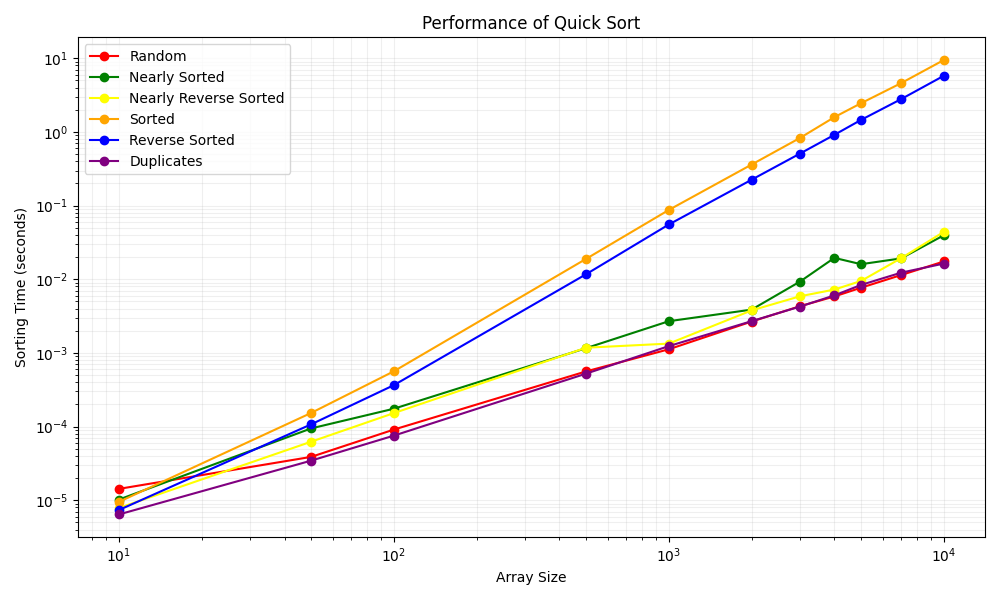
\includegraphics[width=.9\linewidth]{sorting_performance_quick_sort.png}
\caption{\label{fig:org9660dbe}Performance of Quick Sort across different input types}
\end{figure}

Based on the measurement results, Quick Sort demonstrates excellent performance for random arrays and arrays with duplicates, consistently being among the fastest algorithms for these input types. However, its performance degrades significantly for sorted and reverse-sorted arrays, where it exhibits quadratic time complexity. For instance, at array size 10,000, Quick Sort took approximately 9.47 seconds for sorted arrays compared to just 0.017 seconds for random arrays. This confirms the theoretical weakness of Quick Sort when dealing with already sorted or nearly sorted data.
\subsection{Merge Sort}
\label{sec:orga2d20a6}
Merge Sort is another divide-and-conquer algorithm that divides the input array into two halves, recursively sorts them, and then merges the sorted halves. The key operation is the merging of two sorted subarrays into a single sorted array. Merge Sort has a consistent O(n log n) time complexity for all cases, making it reliable across different input types.
\subsubsection{Implementation}
\label{sec:org8d338da}
\begin{listing}[htbp]
\begin{Code}
\begin{Verbatim}
\color{EFD}\EFk{def} \EFf{merge}(arr, left, mid, right):
    \EFv{n1} \textcolor[HTML]{000000}{=} mid \textcolor[HTML]{000000}{-} left \textcolor[HTML]{000000}{+} 1
    \EFv{n2} \textcolor[HTML]{000000}{=} right \textcolor[HTML]{000000}{-} mid
    \EFcd{\# }\EFc{Create temp arrays}
    \EFv{L} \textcolor[HTML]{000000}{=} [0] \textcolor[HTML]{000000}{*} n1
    \EFv{R} \textcolor[HTML]{000000}{=} [0] \textcolor[HTML]{000000}{*} n2
    \EFcd{\# }\EFc{Copy data to temp arrays L[] and R[]}
    \EFk{for} i \EFk{in} \EFb{range}(n1):
        \EFv{L}[i] \textcolor[HTML]{000000}{=} arr[left \textcolor[HTML]{000000}{+} i]
    \EFk{for} j \EFk{in} \EFb{range}(n2):
        \EFv{R}[j] \textcolor[HTML]{000000}{=} arr[mid \textcolor[HTML]{000000}{+} 1 \textcolor[HTML]{000000}{+} j]
    \EFv{i} \textcolor[HTML]{000000}{=} 0  \EFcd{\# }\EFc{Initial index of first subarray}
    \EFv{j} \textcolor[HTML]{000000}{=} 0  \EFcd{\# }\EFc{Initial index of second subarray}
    \EFv{k} \textcolor[HTML]{000000}{=} left  \EFcd{\# }\EFc{Initial index of merged subarray}
    \EFcd{\# }\EFc{Merge the temp arrays back}
    \EFcd{\# }\EFc{into arr[left..right]}
    \EFk{while} i \textcolor[HTML]{000000}{<} n1 \EFk{and} j \textcolor[HTML]{000000}{<} n2:
        \EFk{if} L[i] \textcolor[HTML]{000000}{<=} R[j]:
            \EFv{arr}[k] \textcolor[HTML]{000000}{=} L[i]
            \EFv{i} \textcolor[HTML]{000000}{+=} 1
        \EFk{else}:
            \EFv{arr}[k] \textcolor[HTML]{000000}{=} R[j]
            \EFv{j} \textcolor[HTML]{000000}{+=} 1
        \EFv{k} \textcolor[HTML]{000000}{+=} 1
    \EFcd{\# }\EFc{Copy the remaining elements of L[],}
    \EFcd{\# }\EFc{if there are any}
    \EFk{while} i \textcolor[HTML]{000000}{<} n1:
        \EFv{arr}[k] \textcolor[HTML]{000000}{=} L[i]
        \EFv{i} \textcolor[HTML]{000000}{+=} 1
        \EFv{k} \textcolor[HTML]{000000}{+=} 1
    \EFcd{\# }\EFc{Copy the remaining elements of R[],}
    \EFcd{\# }\EFc{if there are any}
    \EFk{while} j \textcolor[HTML]{000000}{<} n2:
        \EFv{arr}[k] \textcolor[HTML]{000000}{=} R[j]
        \EFv{j} \textcolor[HTML]{000000}{+=} 1
        \EFv{k} \textcolor[HTML]{000000}{+=} 1
    \EFk{return}


\EFk{def} \EFf{merge\_sort\_rec}(arr, left, right):
    \EFk{if} left \textcolor[HTML]{000000}{<} right:
        \EFv{mid} \textcolor[HTML]{000000}{=} (left \textcolor[HTML]{000000}{+} right) \textcolor[HTML]{000000}{//} 2
        merge\_sort\_rec(arr, left, mid)
        merge\_sort\_rec(arr, mid \textcolor[HTML]{000000}{+} 1, right)
        merge(arr, left, mid, right)
    \EFk{return}


\EFk{def} \EFf{merge\_sort}(arr):
    merge\_sort\_rec(arr, 0, \EFb{len}(arr)\textcolor[HTML]{000000}{-}1)
\end{Verbatim}
\end{Code}
\caption{\label{lst:orgff19348}Implementation of Merge Sort}
\end{listing}
\subsubsection{Results}
\label{sec:orgca32068}
\begin{figure}[htbp]
\centering
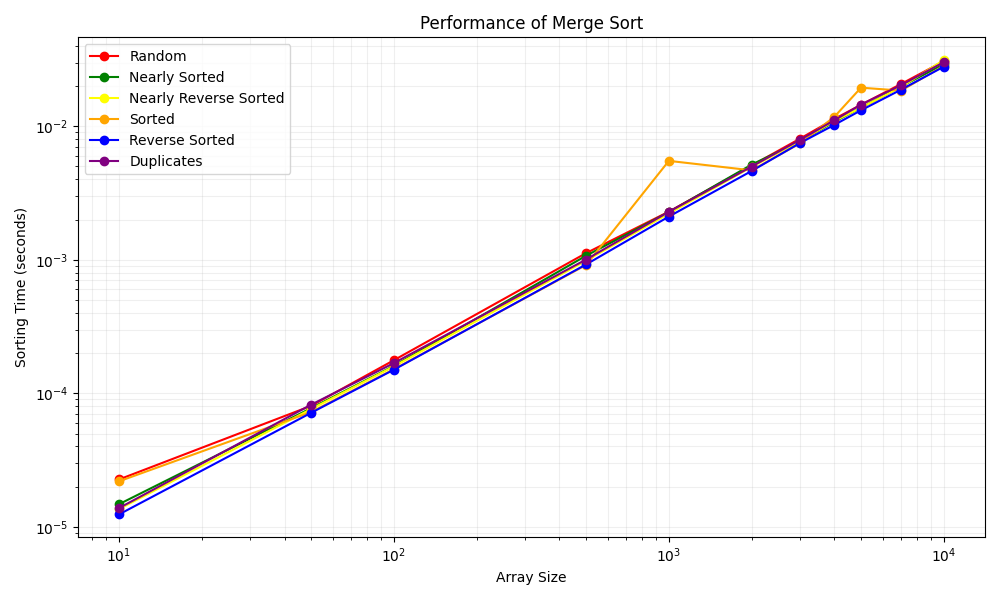
\includegraphics[width=.9\linewidth]{sorting_performance_merge_sort.png}
\caption{\label{fig:org017c9a1}Performance of Merge Sort across different input types}
\end{figure}

The measurement results show that Merge Sort maintains consistent performance across all input types, with execution times clustering closely together regardless of the array's initial arrangement. This stability makes Merge Sort particularly valuable when predictable performance is required. For example, at array size 10,000, Merge Sort's execution time ranges from 0.028 to 0.031 seconds across different input types, demonstrating its stability. However, it's generally not the fastest algorithm for any particular input type, usually being outperformed by Quick Sort for random arrays and by Smart Sort for sorted arrays.
\subsection{Heap Sort}
\label{sec:org9e7de18}
Heap Sort uses a binary heap data structure to sort elements. It first builds a max-heap from the input data, then repeatedly extracts the maximum element from the heap and rebuilds the heap until all elements are extracted. Heap Sort has a consistent O(n log n) time complexity in all cases and requires O(1) extra space.
\subsubsection{Implementation}
\label{sec:org372ddf9}
\begin{listing}[htbp]
\begin{Code}
\begin{Verbatim}
\color{EFD}\EFk{def} \EFf{heapify}(arr, n, i):
    \EFv{largest} \textcolor[HTML]{000000}{=} i
    \EFv{l\_idx} \textcolor[HTML]{000000}{=} 2 \textcolor[HTML]{000000}{*} i \textcolor[HTML]{000000}{+} 1
    \EFv{r\_idx} \textcolor[HTML]{000000}{=} 2 \textcolor[HTML]{000000}{*} i \textcolor[HTML]{000000}{+} 2
    \EFk{if} l\_idx \textcolor[HTML]{000000}{<} n \EFk{and} arr[l\_idx] \textcolor[HTML]{000000}{>} arr[largest]:
        \EFv{largest} \textcolor[HTML]{000000}{=} l\_idx
    \EFk{if} r\_idx \textcolor[HTML]{000000}{<} n \EFk{and} arr[r\_idx] \textcolor[HTML]{000000}{>} arr[largest]:
        \EFv{largest} \textcolor[HTML]{000000}{=} r\_idx
    \EFk{if} largest \textcolor[HTML]{000000}{!=} i:
        \EFv{arr}[\EFv{i}], \EFv{arr}[largest] \textcolor[HTML]{000000}{=} arr[largest], arr[i]  \EFcd{\# }\EFc{Swap}
        heapify(arr, n, largest)


\EFk{def} \EFf{heap\_sort}(arr):
    \EFv{n} \textcolor[HTML]{000000}{=} \EFb{len}(arr)
    \EFk{for} i \EFk{in} \EFb{range}(n \textcolor[HTML]{000000}{//} 2 \textcolor[HTML]{000000}{-} 1, \textcolor[HTML]{000000}{-}1, \textcolor[HTML]{000000}{-}1):
        heapify(arr, n, i)
    \EFk{for} i \EFk{in} \EFb{range}(n \textcolor[HTML]{000000}{-} 1, 0, \textcolor[HTML]{000000}{-}1):
        \EFv{arr}[0], \EFv{arr}[i] \textcolor[HTML]{000000}{=} arr[i], arr[0]
        heapify(arr, i, 0)
    \EFk{return}
\end{Verbatim}
\end{Code}
\caption{\label{lst:org3d0adf4}Implementation of Heap Sort}
\end{listing}
\subsubsection{Results}
\label{sec:org2a7d763}
\begin{figure}[htbp]
\centering
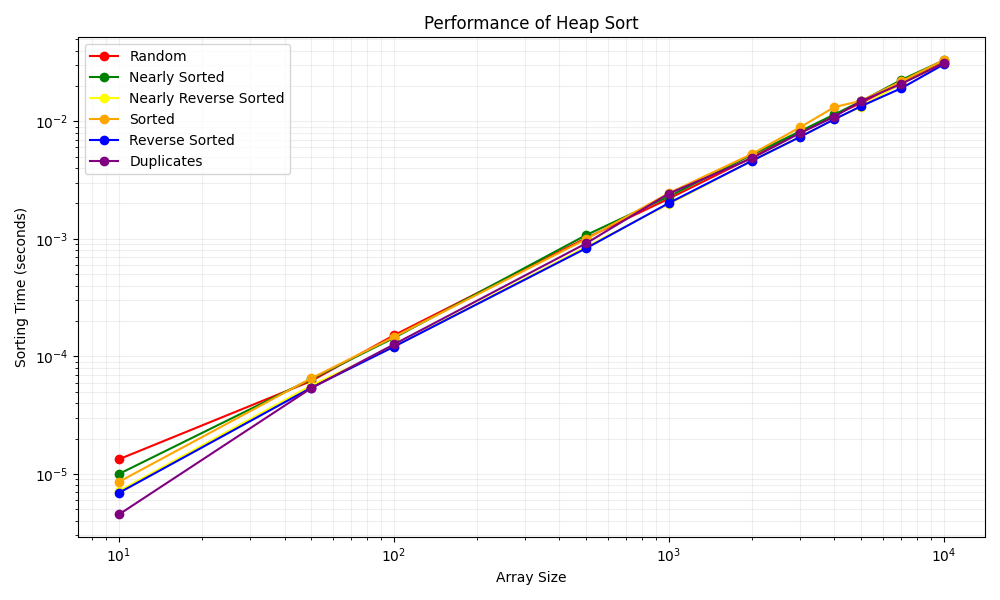
\includegraphics[width=.9\linewidth]{sorting_performance_heap_sort.png}
\caption{\label{fig:orgb73fac1}Performance of Heap Sort across different input types}
\end{figure}

The measurement results indicate that Heap Sort exhibits consistent performance across all input types, similar to Merge Sort. It performs particularly well for nearly reverse-sorted arrays, where it often outperforms other algorithms. For example, at array size 10,000, Heap Sort took approximately 0.031 seconds for nearly reverse-sorted arrays, making it competitive with Merge Sort. However, it's generally slower than Quick Sort for random arrays and significantly slower than Smart Sort for sorted arrays.
\subsection{Patience Sort}
\label{sec:orgb896780}
Patience Sort is inspired by the card game Patience (Solitaire). It creates piles of cards and uses a merge operation similar to Merge Sort to combine them. The algorithm has a worst-case time complexity of O(n\(^{2}\)) if unoptimized, and  O(n log n) if optimized with a heap for merging. It performs particularly well on partially sorted data, and has a best case O(n) complexity when the array is sortred in reverse.
\subsubsection{Implementation}
\label{sec:orgbbf4209}
\begin{listing}[htbp]
\begin{Code}
\begin{Verbatim}
\color{EFD}\EFk{def} \EFf{patience\_sort}(collection):
    \EFv{piles} \textcolor[HTML]{000000}{=} []  \EFcd{\# }\EFc{A list of piles of cards}
    \EFk{for} item \EFk{in} collection:
        \EFv{new\_pile} \textcolor[HTML]{000000}{=} [item]
        \EFk{for} pile \EFk{in} piles:
            \EFk{if} item \textcolor[HTML]{000000}{<} pile[\textcolor[HTML]{000000}{-}1]:  \EFcd{\# }\EFc{If the item is smaller than the last card in the pile}
                pile.append(item)  \EFcd{\# }\EFc{Add the item to the pile}
                \EFk{break}
        \EFk{else}:
            piles.append(new\_pile)  \EFcd{\# }\EFc{If the item is larger than all the piles, create a new pile for it}

    \EFv{sorted\_list} \textcolor[HTML]{000000}{=} []  \EFcd{\# }\EFc{A list of sorted cards}
    \EFk{while} piles:
        \EFv{smallest\_pile} \textcolor[HTML]{000000}{=} \EFb{min}(piles, key\textcolor[HTML]{000000}{=}\EFk{lambda} pile: pile[\textcolor[HTML]{000000}{-}1])  \EFcd{\# }\EFc{Find the smallest pile by comparing the last cards}
        sorted\_list.append(smallest\_pile.pop())  \EFcd{\# }\EFc{Remove the last card from the smallest pile and add it to the sorted list}
        \EFk{if} \EFk{not} smallest\_pile:  \EFcd{\# }\EFc{If the smallest pile is empty, remove it from the list of piles}
            piles.remove(smallest\_pile)

    \EFk{for} i \EFk{in} \EFb{range}(\EFb{len}(collection)):
        \EFv{collection}[i] \textcolor[HTML]{000000}{=} sorted\_list[i]

    \EFk{return}
\end{Verbatim}
\end{Code}
\caption{\label{lst:orgfa49fb2}Implementation of Patience Sort}
\end{listing}
\subsubsection{Results}
\label{sec:orgbab5c7a}
\begin{figure}[htbp]
\centering
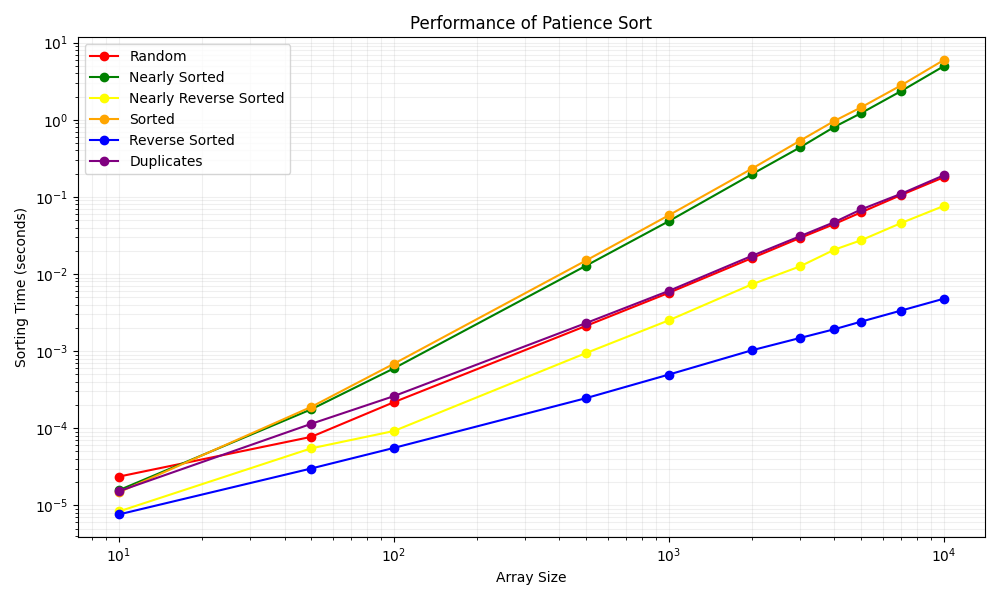
\includegraphics[width=.9\linewidth]{sorting_performance_patience_sort.png}
\caption{\label{fig:org3f773f3}Performance of Patience Sort across different input types}
\end{figure}

Patience Sort demonstrates interesting performance characteristics across different input types. It performs reasonably well for random arrays and arrays with duplicates, although not as fast as Quick Sort or Smart Sort. However, it struggles significantly with sorted and nearly sorted arrays, showing exponential growth in execution time as the array size increases. For instance, at array size 10,000, Patience Sort took approximately 5.95 seconds for sorted arrays and 4.95 seconds for nearly sorted arrays, making it the second slowest algorithm for these input types. Interestingly, Patience Sort performs well on reverse-sorted arrays, being the second fastest algorithm after Smart Sort for this input type, confirming the theory around it.
\subsection{Smart Sort}
\label{sec:orgfe2e1a1}
Smart Sort is hybrid sorting algorithm that adapts its strategy based on the input characteristics, it demonstrates exceptional performance in certain scenarios, particularly for sorted and reverse-sorted arrays.
It uses Heap sort for arrays smaller than 500 elements, and merge for the rest in the case of nearly sorted arrays. For all the other cases it uses QuickSort.
\subsubsection{Implementation}
\label{sec:org1e786df}
\begin{listing}[htbp]
\begin{Code}
\begin{Verbatim}
\color{EFD}\EFk{def} \EFf{smart\_sort}(arr):
    \EFv{size} \textcolor[HTML]{000000}{=} \EFb{len}(arr)

    \EFcd{\# }\EFc{Handle empty or single element arrays}
    \EFk{if} size \textcolor[HTML]{000000}{<=} 1:
        \EFk{return}

    \EFcd{\# }\EFc{Check if array is already sorted}
    \EFk{if} is\_sorted(arr):
        \EFk{return}

    \EFcd{\# }\EFc{Check if array is reverse sorted}
    \EFk{if} is\_sorted(arr[::\textcolor[HTML]{000000}{-}1]):
        \EFcd{\# }\EFc{Reverse the array in-place}
        \EFv{left}, \EFv{right} \textcolor[HTML]{000000}{=} 0, \EFb{len}(arr) \textcolor[HTML]{000000}{-} 1
        \EFk{while} left \textcolor[HTML]{000000}{<} right:
            \EFv{arr}[\EFv{left}], \EFv{arr}[right] \textcolor[HTML]{000000}{=} arr[right], arr[left]
            \EFv{left} \textcolor[HTML]{000000}{+=} 1
            \EFv{right} \textcolor[HTML]{000000}{-=} 1
        \EFk{return}

    \EFcd{\# }\EFc{For very small arrays (size < 50)}
    \EFk{if} size \textcolor[HTML]{000000}{<} 50:
        quick\_sort(arr)
        \EFk{return}

    \EFv{nearly\_sorted} \textcolor[HTML]{000000}{=} is\_nearly\_sorted\_v2(arr)

    \EFk{if} nearly\_sorted:
        \EFcd{\# }\EFc{For arrays size 50-500}
        \EFk{if} size \textcolor[HTML]{000000}{<=} 500:
            heap\_sort(arr)
            \EFk{return}

        \EFcd{\# }\EFc{For larger arrays (size >= 500)}
        \EFk{else}:
            merge\_sort(arr)
            \EFk{return}

    quick\_sort(arr)
    \EFk{return}
\end{Verbatim}
\end{Code}
\caption{Implementation of Smart Sort}
\end{listing}
\subsubsection{Results}
\label{sec:org2e46eef}
\begin{figure}[htbp]
\centering
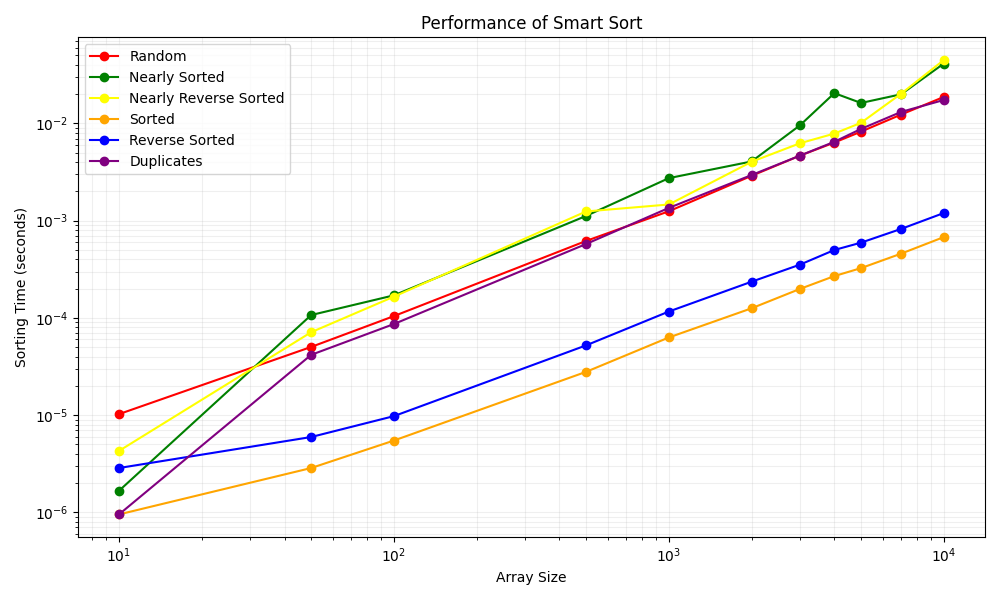
\includegraphics[width=.9\linewidth]{sorting_performance_smart_sort.png}
\caption{\label{fig:orgf3a7cb5}Performance of Smart Sort across different input types}
\end{figure}

The measurement results confirm that Smart Sort is exceptionally efficient for sorted and reverse-sorted arrays, outperforming all other algorithms by several orders of magnitude. For example, at array size 10,000, Smart Sort took just 0.000678 seconds for sorted arrays and 0.001199 seconds for reverse-sorted arrays, while the next fastest algorithm took over 0.027 seconds. This is because Smart Sort includes optimization for detecting already sorted sequences. For random arrays and arrays with duplicates, Smart Sort performs similarly to Quick Sort, being slightly slower but still very efficient. However, for nearly sorted arrays, Smart Sort is somewhat slower than Merge Sort and Heap Sort at larger array sizes.
Even if the Smart Sort we implemented picks the best sort for the job, the part of analyzing the input slows it down, making it 2nd best performing in most cases.
\section{Conclusions}
\label{sec:orgcaa627c}

Based on the empirical analysis of the five sorting algorithms across different input types and sizes, we can draw the following conclusions:

\begin{enumerate}
\item \textbf{Algorithm Selection Depends on Input Characteristics}: No single algorithm performs best across all input types. The choice of sorting algorithm should be informed by the expected characteristics of the input data.

\item \textbf{Quick Sort}: Excels with random arrays and arrays with duplicates, making it a good general-purpose choice when the input is expected to be unsorted. However, it performs poorly on sorted or nearly sorted arrays, exhibiting quadratic time complexity in these cases.

\item \textbf{Merge Sort}: Provides consistent performance across all input types, making it reliable when predictable execution time is required. While not the fastest in most scenarios, its stability makes it valuable for applications where worst-case performance is a concern.

\item \textbf{Heap Sort}: Similar to Merge Sort in offering consistent performance across input types. It performs particularly well for nearly reverse-sorted arrays but is generally outperformed by other algorithms in specific scenarios.

\item \textbf{Patience Sort}: Demonstrates good performance for random arrays and reverse-sorted arrays but struggles significantly with sorted and nearly sorted arrays. Its use should be limited to scenarios where the input is known to be random or reverse-sorted.

\item \textbf{Smart Sort}: Shows exceptional performance for sorted and reverse-sorted arrays, suggesting sophisticated detection of already sorted sequences. It performs comparably to Quick Sort for random arrays and arrays with duplicates, making it a versatile choice when the input characteristics are known.

\item \textbf{Scaling Behavior}: All algorithms show the expected O(n log n) scaling for random arrays, as evidenced by the linear relationship on the log-log plots. However, Quick Sort and Patience Sort exhibit quadratic scaling for sorted arrays, confirming their theoretical worst-case behavior.

\item \textbf{Practical Takeaways}:
\begin{itemize}
\item For general-purpose sorting with unknown input characteristics, Merge Sort provides the most consistent performance.
\item When sorting efficiency is critical and the input is likely to be random, Quick Sort is the best choice.
\item even if the SmartSort we implemented picks the best sort for the job, the part of analyzing the input slows it down, making it 2nd best performing in most cases.
\item For memory-constrained environments, Heap Sort provides good performance with minimal additional space requirements.
\end{itemize}
\end{enumerate}

The results imply the importance of understanding both the theoretical properties of sorting algorithms and their empirical performance characteristics when selecting an algorithm for a specific application.
\end{document}
